\subsection{Nivel de abstracción 1: Módulos principales}

  \paragraph{}El nivel de abstracción 1 muestra una visión general de los
  módulos principales de los que se compone la aplicación: Administrador
  principal, Administrador de centro, Asesores y Alumnos.

  \begin{description}
   \item[Módulo de Administrador principal] Este módulo se encargará de
   crear y mantener toda la estructura básica de la aplicación, gestionando
   al resto de usuarios del sistema, así como los distintos centros,
   titulaciones y asignaturas que se establezcan durante los distintos cursos
   académicos.

   \paragraph{}Recibirá flujos de entrada de información por parte de las
   entidades externas Teclado, Ratón y Sistema. A su vez, también recibirá
   flujos de entrada del almacén Unidad de almacenamiento.

   \paragraph{}Producirá flujos de salida de información tales como mensajes de
   información consultada, mensajes de error, resultados de las operaciones e
   información impresa.

   \paragraph{}La interacción con la base de datos BBDD Asesoría Académica se
   realizará mediante un flujo bidireccional, realizando consultas a la base de
   datos para extraer datos (flujo de entrada) y realizando consultas de
   inserción, modificación y actualización en la base de datos (flujo de
   salida).

   \item[Módulo de Administrador de centro] Este módulo se encargará de
   crear y mantener toda la información relativa a los distintos centros
   que compongan el sistema, gestionando a los usuarios teniendo en cuenta el
   centro al que pertenecen, así como las distintas titulaciones y asignaturas
   que dispongan dichos centros, establecidos durante los distintos cursos
   académicos.

   \paragraph{}Recibirá flujos de entrada de información por parte de las
   entidades externas Teclado y Ratón. A su vez, también recibirá flujos de
   entrada del almacén Unidad de almacenamiento.

   \paragraph{}Producirá flujos de salida de información tales como mensajes de
   información consultada, mensajes de error, resultados de las operaciones e
   información impresa.

   \paragraph{}La interacción con la base de datos BBDD Asesoría Académica se
   realizará mediante un flujo bidireccional, realizando consultas a la base de
   datos para extraer datos (flujo de entrada) y realizando consultas de
   inserción, modificación y actualización en la base de datos (flujo de
   salida).

   \item[Módulo de Asesores] Este módulo se encargará de gestionar a los alumnos
   a los que se preste asesoría, además de crear y mantener las distintas
   plantillas de entrevistas de asesor personales. También será el encargado
   de convocar reuniones en las que participarán los asesores y los alumnos
   que correspondan.

   \paragraph{}Recibirá flujos de entrada de información por parte de las
   entidades externas Teclado y Ratón. A su vez, también recibirá flujos de
   entrada del almacén Unidad de almacenamiento.

   \paragraph{}Producirá flujos de salida de información tales como mensajes de
   información consultada, mensajes de error, resultados de las operaciones e
   información impresa.

   \paragraph{}La interacción con la base de datos BBDD Asesoría Académica se
   realizará mediante un flujo bidireccional, realizando consultas a la base de
   datos para extraer datos (flujo de entrada) y realizando consultas de
   inserción, modificación y actualización en la base de datos (flujo de
   salida).

   \item[Módulo de Alumnos]
  \end{description}

  \paragraph{}La figura \ref{diagramaNivel1} muestra el nivel de abstracción 1.

        \begin{figure}[!ht]
            \begin{center}
            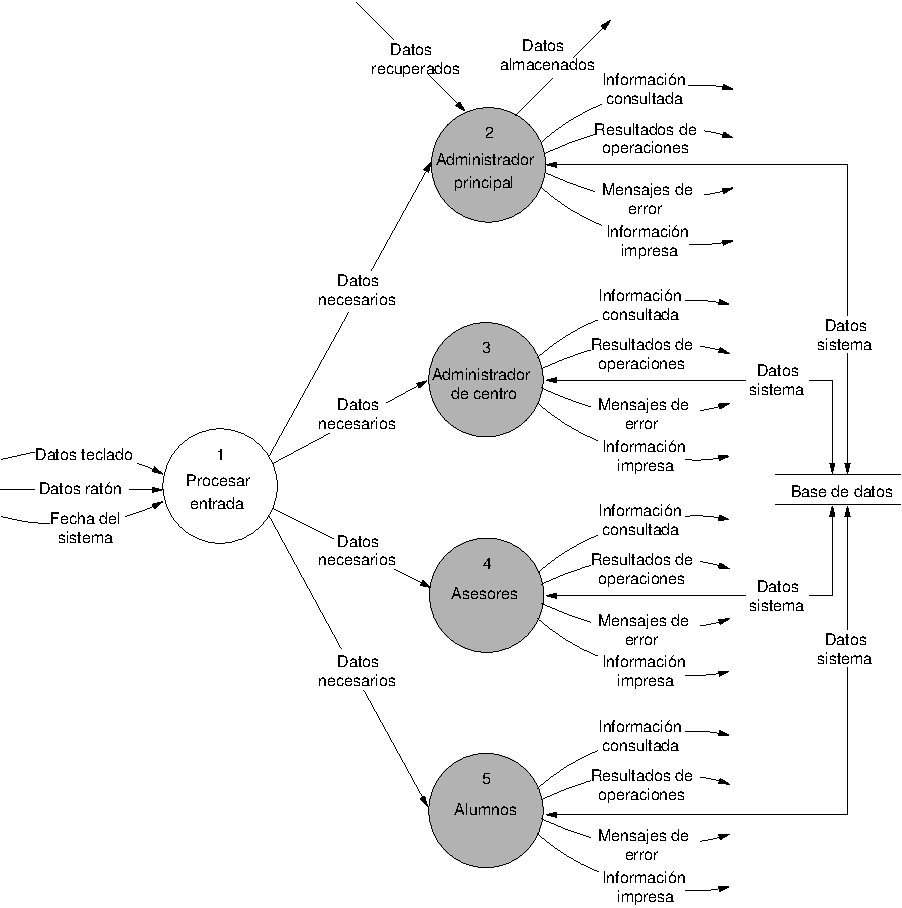
\includegraphics[]{08.Analisis_Funcional/8.2.DFDs/Niveles/Diagramas/nivel1.pdf}
            \caption{Nivel de abstracción 1: Módulos principales.}
            \label{diagramaNivel1}
            \end{center}
         \end{figure}